   %
% IEEE Transactions on Microwave Theory and Techniques example
% Tibault Reveyrand - http://www.microwave.fr
%
% http://www.microwave.fr/LaTeX.html
% ---------------------------------------



% ================================================
% Please HIGHLIGHT the new inputs such like this :
% Text :
%  \hl{comment}
% Aligned Eq. 
% \begin{shaded}
% \end{shaded}
% ================================================



\documentclass[journal]{IEEEtran}
%\usepackage[retainorgcmds]{IEEEtrantools}
%\usepackage{bibentry}  
\usepackage{xcolor,soul,framed} %,caption
\usepackage[spanish]{babel}
\colorlet{shadecolor}{yellow}
% \usepackage{color,soul}
\usepackage[pdftex]{graphicx}
\graphicspath{{../pdf/}{../jpeg/}}
\DeclareGraphicsExtensions{.pdf,.jpeg,.png}

\usepackage[cmex10]{amsmath}
%Mathabx do not work on ScribTex => Removed
%\usepackage{mathabx}
\usepackage{array}
\usepackage{mdwmath}
\usepackage{mdwtab}
\usepackage{eqparbox}
\usepackage{url}

%\hyphenation{op-tical net-works semi-conduc-tor}

%\bstctlcite{IEEE:BSTcontrol}


%=== TITLE & AUTHORS ====================================================================
\begin{document}
\title{Visi\'on Computacional, Aplicaci\'on y Estado de Arte}
\author{Medina Lopez ,Jahir.  Pacheco Miranda ,Miguel.\\
    jahir.medina@unitru.edu.pe | jpacheco@unitru.edu.pe\\
    Facultad de Ciencias Fisica y Matematicas, Informatica}



% The paper headers
\markboth{Universidad Nacional de Trujillo. | Medina \& Pacheco : \textbf{Procesamiento de Im\'agenes, Aplicaciones}}
{Medina \& Pacheco : Visi\'on Computacional, Aplicaciones}



% ====================================================================
\maketitle



% === ABSTRACT ====================================================================
% =================================================================================
\begin{abstract}
%\boldmath
El presente articulo recopila las aplicaciones y avances del \'area de la inform\'atica y electr\'onica denominada Visi\'on Computacional, considerando como marco referente el estado de arte del mismo.

Si bien en el pasado \cite{mit_csail} la \textit{V.C.}(siglas de visi\'on computacional) se encontraba alejado del consumidor, es decir, las aplicaciones relacionadas al \'area ten\'ian un factor acad\'emico u exploratorio; el distanciamiento era tal
que la universidades deb\'ian tener departamentos especializados, haciendo pr\'acticamente imposible una aproximaci\'on amateur a este campo de estudio.
\\
En la actualidad, con el avance de la electr\'onica, el perfeccionamiento de m\'etodos matematismos mas complejos y el mas com\'un uso de frameworks y librer\'ias especializadas ~\cite{Keim2008} (OpenCV, CUDA, TensorFlow); los progresos en investigaci\'on rivaliza en velcidad con su capacidad para generar productos finales \cite{majoreports} (Google Glass, Microsft Hololens, Tesla Self Driving Cars).

Sin embargo, a mayor uso y mejor desempe\~no de las aplicaciones del \textit{PDI} aparecen nuevos problemas t\'ecnicos.

\end{abstract}


% === KEYWORDS ====================================================================
% =================================================================================
\ \\
\ \\

\begin{IEEEkeywords}
    Visi\'on Computacional, Aprendizaje de Maquina, T\'ecnicas no Supevisionadas, Realidad Aumentada
\end{IEEEkeywords}

% page as needed:
% \ifCLASSOPTIONpeerreview
% \begin{center} \bfseries EDICS Category: 3-BBND \end{center}
% \fi
%
% For peerreview papers, this IEEEtran command inserts a page break and
% creates the second title. It will be ignored for other modes.
\IEEEpeerreviewmaketitle


% ====================================================================
% ====================================================================
% ====================================================================



% === I. INTRODUCTION =============================================================
% =================================================================================
\section{Introducci\'on}


La visi\'on computacional es el \'area que mas r\'apidamente a crecido en los \'ultimos a�os, en
t\'erminos de aplicaci\'on e investigaci\'on, si bien es cierto parte de su desarrollo esta relacionado con el avance de las rede neuronales artificiales y t\'ecnicas de aprendizaje autom\'atico, el an\'alisis cl\'asico a disminuido
pero no desaparecido\cite{majoreports}.
\\
La visi\'on computacional cl\'asica (an\'alisis de complejidad algor\'itmica, optimizaci\'on de recursos, etc) \cite{opencv_manual} resulta importante al momento de explicar los formalismos detr\'as de las t\'ecnicas mas actuales. Por ejemplo, explicar una t\'ecnica que reside sobre una red neuronal profunda resultar\'ia en una serie de tecnicismos sobre camadas, funciones de activaci\'on, probabilidad de \textit{dropout} y muchas jerga obtusa; sin dar lugar a consideraciones directas : �Que caracter\'isticas extrae? , �con que probabilidad selecciona cada area?, �es eficiente en producci\'on?.
\\
Considerando todo esto, es claro que el Procesamiento digital de im\'agenes moderno es una mezcla de t\'ecnicas antiguas y nuevas, pero su aplcacion en la industria o servicios al publico es af\'in con el descongelamiento de la inteligencia artifical. Desde finales de los 80's, donde la venta de \textit{scaners}con chips orientados al reconocimieto grafico de caracteres marcaba un comienzo en la industria del hardware orientado al procesamiento digital de im\'agenes y visi\'on computacional. Este progreso continua hasta llegar a los actuales chips de IA  y mejoramiento fotogr\'afico embebidos en los celulares Huaweii o chips Nvidia 
Tegra~\cite{nvidia_tegra} .

La facilidad con la que el hardware a mejorado el desempe�o de los algoritmos cl\'asicos y los resultados de las t\'ecnicas modernas sobrepasaron o crearon nuevos enfoques, se ha conseguido alejarse del tele-procesamiento a sistemas embebidos mas robustos, por ejemplo el Curiosity Rover viajo equipado de un mini-cl\'uster dual de chips PowerPC (elegidos por su muy bajo consumo energ\'etico) \cite{Matthies2007}.

\begin{figure}
	\begin{center}
		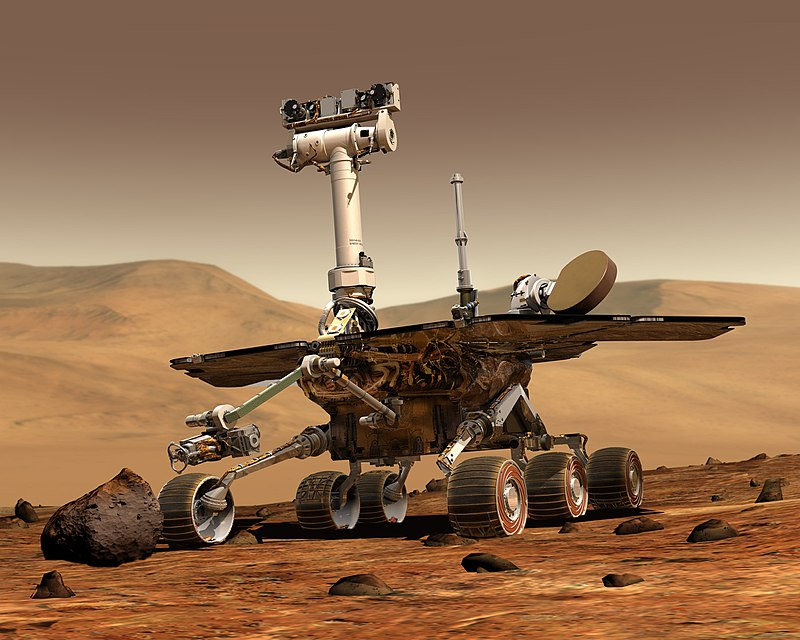
\includegraphics[width=3.5in]{pdf/NASA_Mars_Rover.jpg}\\
		\caption{Curiosity Rover}
	\end{center}
\end{figure}

% === II. Harmonically-Terminated Power Rectifier Analysis ========================
% =================================================================================
\section{Aplicaciones}

\subsection{Red Y.O.L.O.}

En im\'agenes, You Only Look Once (YOLO) \cite{redmon} es un m\'etodo de detecci\'on de objetos de enfoque avanzado. YOLO aplica una sola CNN a toda la imagen que divide la imagen en grillas. La predicci\'on de los cuadros delimitadores y la puntuaci\'on de confianza respectiva se calculan para cada cuadr\'icula. Estos cuadros delimitadores se analizan seg\'un el puntaje de confianza previsto. La arquitectura de YOLO tiene 24 capas convolucionales y 2 capas completamente conectadas. La arquitectura se muestra en Figura 1.
% Aqui va la figura 2
El algoritmo aplica una red neuronal a una imagen entera redimensionada a 480x480 p\'ixeles. La red divide la imagen en una malla de SxS y presenta cuadros de l\'imites, que son cuadros dibujados alrededor de im\'agenes y probabilidades para cada una de estas regiones. 
% Aqui va la figura 3
El m\'etodo utilizado para generar estas probabilidades es la regresi\'on log\'istica. Los cuadros delimitadores est\'an ponderados por las probabilidades asociadas. Para la predicci\'on de clase, se utilizan clasificadores log\'isticos independientes.
% Aqui va la figura 4
Sin embargo, la regla de un solo objeto limita lo cerca que pueden estar los objetos detectados. Para eso, YOLO tiene algunas limitaciones sobre lo cerca que pueden estar los objetos.
% Aqui va la figura 5
% Conclusiones
En comparaci\'on con los m\'etodos convencionales de detecci\'on de objetos, YOLO tiene ciertas ventajas. 1) En lugar de utilizar el m\'etodo de dos pasos para la clasificaci\'on y localizaci\'on del objeto, YOLO aplica un solo CNN tanto para la clasificaci\'on como para la localizaci\'on del objeto. 2) YOLO puede procesar im\'agenes a aproximadamente 40-90 FPS, por lo que es bastante r\'apido. Esto significa que la transmisi\'on de video se puede procesar en tiempo real, con una latencia insignificante en unos pocos milisegundos. La arquitectura de YOLO lo hace extremadamente r\'apido. Cuando se compara con R-CNN, es 1000 veces m\'as r\'apido y 100 veces m\'as r\'apido que el Faster R-CNN\cite{shinde}.


% =======
% FIG. 01
% =======
\begin{figure}
  \begin{center}
  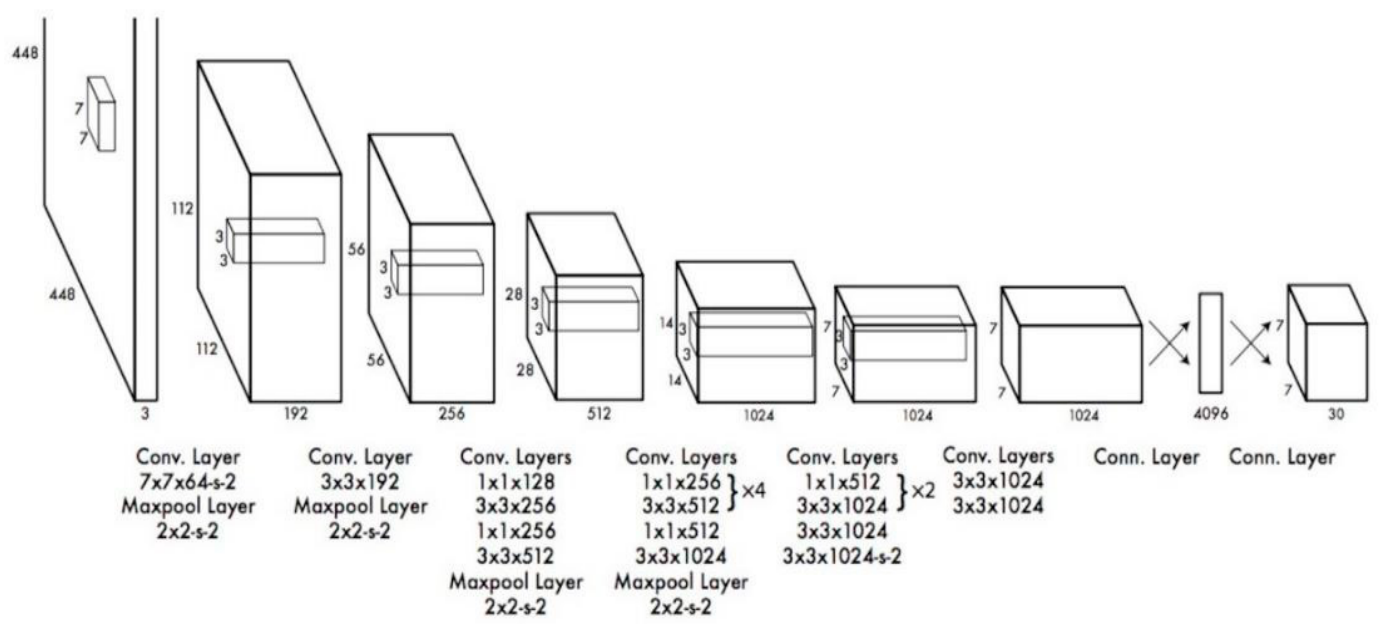
\includegraphics[width=3.5in]{pdf/yolo.png}\\
  \caption{Arquitectura de YOLO.}
  \end{center}
\end{figure}

% =======
% FIG. 02
% =======
\begin{figure}
  \begin{center}
  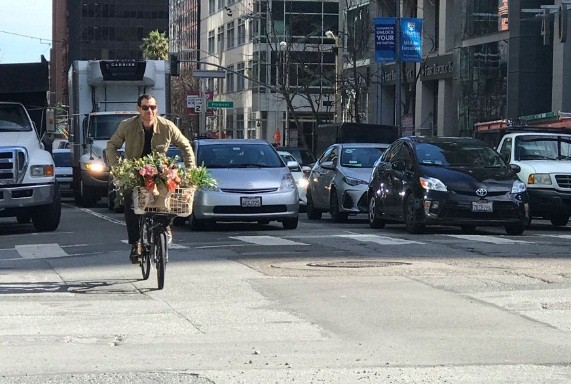
\includegraphics[width=2.0in]{pdf/yoloentrada1.jpg}\\
  \caption{Imagen de Entrada.}
  \end{center}
\end{figure}

% =======
% FIG. 03
% =======
\begin{figure}
  \begin{center}
  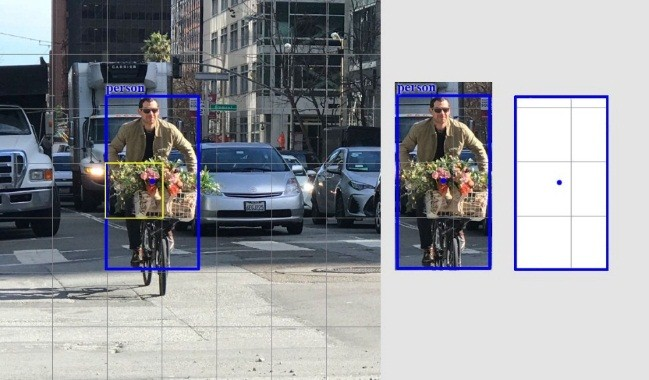
\includegraphics[width=2.0in]{pdf/yoloentrada3.jpg}\\
  \caption{Imagen dividida en una malla SxS.}
  \end{center}
\end{figure}

% =======
% FIG. 04
% =======
\begin{figure}
  \begin{center}
  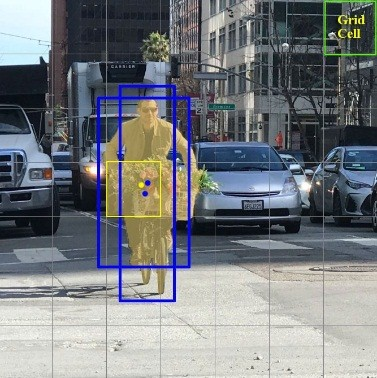
\includegraphics[width=2.0in]{pdf/yoloentrada4.jpg}\\
      \caption{Imagen con cuadros delimitadores.}
  \end{center}
\end{figure}

% =======
% FIG. 05
% =======

\begin{figure}
\begin{center}
  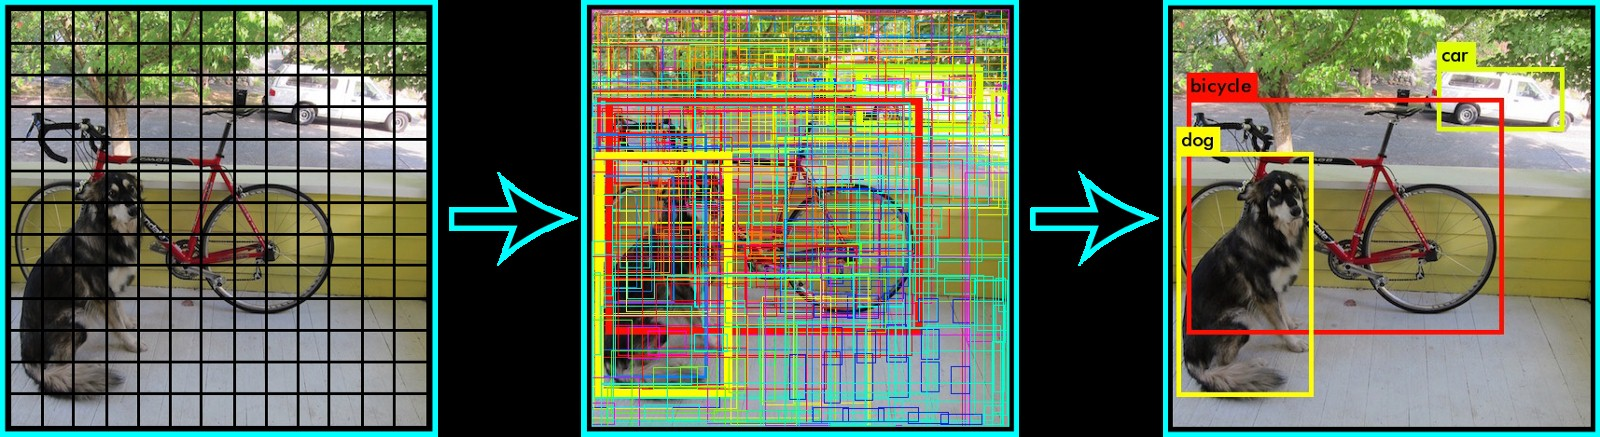
\includegraphics[width=3.5in]{pdf/yoloentrada5.jpg}\\
  \caption{Entrada, Delimitadores, Objetos detectados.}
\end{center}
\end{figure}


\subsection{Lentes de Realidad Virtual}
?La Realidad Virtual es una simulaci\'on interactiva por computador desde el punto de vista del participante, en la cual se sustituye o se aumenta la informaci\'on sensorial que recibe?.
El hecho de que la simulaci\'on sea interactiva es lo que distingue la realidad virtual de una animaci\'on.	
En el caso de la simulaci\'on visual, los algoritmos de s\'intesis de im\'agenes calculan la imagen en el frame buffer con los par\'ametros de c\'amara virtual correspondientes a la posici\'on y orientaci\'on de la cabeza del usuario. La informaci\'on digital del frame buffer se traduce en una se�al de video por la tarjeta gr\'afica y esta se�al se traduce en una imagen f\'isica en el dispositivo de visualizaci\'on.



Perif\'ericos de Realidad Virtual
\begin{itemize}
    \item Dispositivos de Entrada.
    \begin{itemize}
         \item Posicionadores.
         \begin{itemize}
             \item Magn\'eticos.
             \item �pticos
             \item Ac\'usticos.
             \item Mec\'anicos.
             \item De inercia.
         \end{itemize}
         \item Guantes de datos.
         \item Registros de voz.
         \item Dispositivos de entrada 3D.
    \end{itemize}
    \item Dispositivos de Salida.
    \begin{itemize}
        \item Efectos visuales.
        \begin{itemize}
            \item Tecnolog\'ias de visualizaci\'on.
            \item Factores que determinan la calidad de visualizaci\'on.
            \item Dispositivos de visualizaci\'on.
        \end{itemize}
        \item Efectos auditivos.
    \end{itemize}
    
\end{itemize}

%Conclusi\'on
\cite{lee} Concluyen que la revoluci\'on tecnol\'ogica es un signo de nuestros tiempos. Las soluciones proporcionadas por la tecnolog\'ia son aceptadas por la medicina y gradualmente introducidas en la pr\'actica cl\'inica diaria. Este art\'iculo sirve como un resumen contempor\'aneo del entorno virtual y aumentado en el campo de la cirug\'ia de tumores cerebrales.

\subsection{Seguimiento Ocular (Eye Tracking)}
El seguimiento ocular es la tecnolog\'ia para resaltar el movimiento ocular. El dispositivo de implementaci\'on del seguimiento ocular es un rastreador de ojos. Las t\'ecnicas para obtener los datos del movimiento del ojo se pueden concebir en dos tipos: para medir el ojo posici\'on relativa a la cabeza, y para medir la orientaci\'on de los ojos en el espacio, es decir, el "punto de vista"\cite{duchowski}.

El concepto de eye-tracking hace referencia a un conjunto de tecnolog\'ias que permiten monitorizar y registrar la forma en la que una persona mira una determinada escena o imagen, en concreto en qu\'e \'areas fija su atenci\'on, durante cu\'anto tiempo y qu\'e orden sigue en su exploraci\'on visual.

La informaci\'on que se extrae cuando se realiza la tecnolog\'ia de Seguimiento Ocular,es la siguiente:
\begin{enumerate}
    \item D\'onde est\'a mirando una persona de forma continua.
    \item Qu\'e le est\'a llamando la atenci\'on y qu\'e se la llamaba hace un momento.
    \item Qu\'e intenciones tiene esa persona.
    \item El estado de \'animo de esa persona.
    \item Donde debe ir colocado el contenido de valor para el cliente.
    \item Si las se�ales visuales contenidas en la Web conducen de forma eficaz al cliente.
    \item Capacidad del cliente para localizar la informaci\'on que necesita en la Web.
\end{enumerate}

Extra\'ida esta informaci\'on nos servir\'a para:
\begin{itemize}
    \item Para mejorar la Estructura del Contenido.
    \item Mejorar la experiencia de los usuarios en la web.
    \item Guiar al usuario hacia el objetivo de su negocio.
    \item Facilitar los procesos que desea que realice el usuario.
    \item Conseguir Branding en Internet.
    \item Mejorar la imagen de marca a trav\'es del sitio web.

\end{itemize}

%conclusi\'on
Se han hecho experimentos usando un rastreador ?Eyetribe? que tiene una precisi\'on muy satisfactoria y puede producir buenos datos de salida, por lo que \cite{shokishalov} concluye que la pr\'actica de seguimiento ocular proporciona informaci\'on \'util para el an\'alisis e identificaci\'on de vulnerabilidades en los sistemas de gesti\'on mediante documentos electr\'onicos.

% =======
% FIG. 06
% =======

\begin{figure}
\begin{center}
  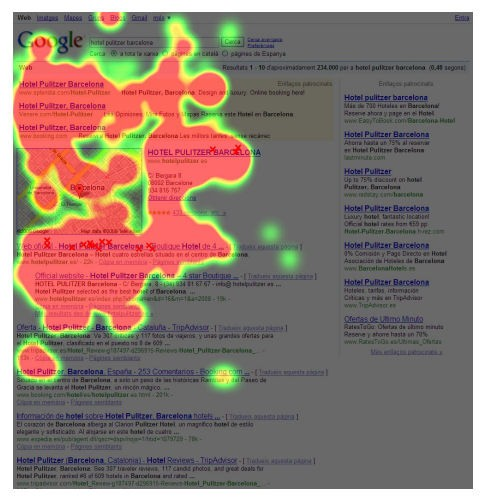
\includegraphics[width=3.5in]{pdf/eyeTracking1.jpg}\\
  \caption{Mapa de calor, mide la intensidad de atencion.}
\end{center}
\end{figure}

\subsection{The Azure Face API}
La API de Azure Face es un servicio cognitivo que proporciona algoritmos para detectar, reconocer y analizar caras humanas en im\'agenes. La capacidad de procesar informaci\'on de rostro humano es importante en muchos escenarios de software diferentes, como seguridad, interfaz de usuario natural, gesti\'on y an\'alisis de contenido de im\'agenes, aplicaciones m\'oviles y rob\'oticas.
La Face API puede detectar rostros humanos en una imagen y devolver las coordenadas del rect\'angulo de sus ubicaciones. Opcionalmente, la detecci\'on facial puede extraer una serie de atributos relacionados con la cara, como postura de la cabeza, sexo, edad, emoci\'on, vello facial y anteojos.

La API Verify realiza una autenticaci\'on contra dos caras detectadas o desde una cara detectada a un objeto de persona. En la pr\'actica, eval\'ua si dos caras pertenecen a la misma persona. Esto es potencialmente \'util en escenarios de seguridad. Para obtener m\'as informaci\'on, consulte la gu\'ia de conceptos de reconocimiento facial o la documentaci\'on de referencia Verificar API.
La API Buscar similares toma una cara de destino y un conjunto de caras candidatas y encuentra un conjunto m\'as peque�o de caras que se parecen m\'as a la cara de destino. Se admiten dos modos de trabajo, matchPerson y matchFace. El modo matchPerson devuelve caras similares despu\'es de filtrar para la misma persona (usando la API Verify). El modo matchFace ignora el filtro de la misma persona y devuelve una lista de caras candidatas similares que pueden o no pertenecer a la misma persona.

\subsection{Deep Fake}

En los \'ultimos 2 a\~nos con el avance en arquitecturas de redes neuronales profundas y el mejoramiento en t\'ecnicas de aumentado de muestras, se consigui\'o generar videos falsos a partir de peque�as muestras de video. Si bien este tipo de trabajos ya exist\'ian , cobro visibilidad con la presentaci�\'on de un trabajo por la Universidad de Washington en el que se reconstru\'ian expresiones faciales que pudieran acomodarse a un discurso especifico (en este caso, un discurso de Barack Obama) \cite{Suwajanakorn_2017}.

\begin{figure}
	\begin{center}
		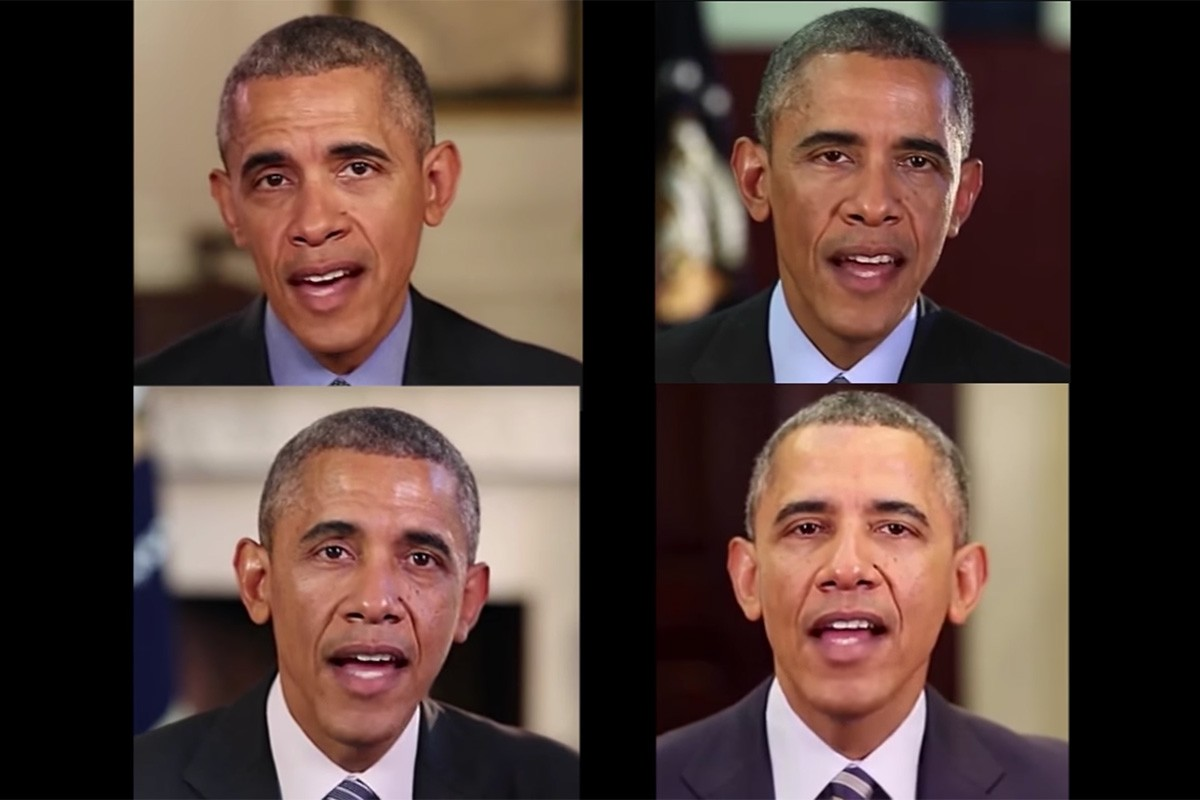
\includegraphics[width=3.5in]{pdf/obama_fake.jpeg}\\
		\caption{Mapa de calor, mide la intensidad de atencion.}
	\end{center}
\end{figure}

\ \\
Sin embargo, trabajos mas recientes, ya no solo facilitan la sincronizaci\'on de expresiones faciales o el modelado 3D apartir una imagen plana \cite{DBLP:journals/corr/JacksonBAT17}, sino la creaci\'on de modelos 3D  din\'amicos \cite{Berger2019}.
\\
Es importante considerar que todo esto es posible no tanto por las redes neuronales en si, sino por las t\ 'ecnicas de incremento artificial de datos, un \'area si bien relacionada a la vision computacional, es no dependiente.
\\
En el futuro \textit{\textbf{SIGGRAPH 2019}} dar\'a debut mas de 4 papers asociado a t\'ecnicas de generaci\'on de video animaci\'on, creaci\'on de cuadros intermedio e iluminaci\'on din\'amica. \cite{youtube_sig2019}


\section{Conclusiones}

Uno de los principales motivos por el cual casi todas , por no generalizar, las aplicaciones y t\'ecnicas de visi\'on computacional actuales dependen de las redes neuronales, recae en su \textit{facilidad} de implementaci\'on (se construye la arquitectura pero no mas).
\\
Consideremos la Red Y.O.L.O, las camadas de convoluci\'on aplican t\'ecnicas cl\'asicas pero la magia sucede en las interconexiones entre neuronas, donde se ajustan pesos y otras variables asociadas la Red como un todo, convirtiendo una red de nodos que suman y restan valores en una funci\'on gigante con forma de grafo.
\\
Mientras en las t\'ecnicas cl\'asicas las funciones aplicadas a las im\'agenes (que no son mas que datos) deb\'ian ser escritas , demostradas y probadas de forma anal\'itica; tal que el dominio y el rango siempre pasen por una funci\'on matem\'atica formal.
\\
Lo que ocurre en las redes neuronales es que suplantan esta funci\'on anal\'itica por una funci\'on param\'etrica, y son estos par\'ametros los que permiten encontrar la mejor funci\'on que sea capaz de llevar del dominio a rango (ejm. im\'agenes a caracter\'isticas).
\\
Se remplazo la b\'usqueda \textit{manual} de una funci\'on m\'agica capaz de cumplir con nuestro objetivo por una b\'usqueda \textit{autom\'atica} (de ah\'i el nombre aprendizaje de maquina, pues es un proceso iterativo).
\\
Finalmente, para estas ultimas t\'ecnicas, en las que los datos son vitales, no se debe olvidar la calidad de los mismos. No todos los datos son dominios y no todos los objetivos son rangos, esto debe ser tomado en consideraci\'on para evitar aplicar t\'ecnicas de avanzada en problemas sencillos.

% if have a single appendix:
%\appendix[Proof of the Zonklar Equations]
% or
%\appendix  % for no appendix heading
% do not use \section anymore after \appendix, only \section*
% is possibly needed

% use appendices with more than one appendix
% then use \section to start each appendix
% you must declare a \section before using any
% \subsection or using \label (\appendices by itself
% starts a section numbered zero.)
%

% ============================================
%\appendices
%\section{Proof of the First Zonklar Equation}
%Appendix one text goes here %\cite{Roberg2010}.

% you can choose not to have a title for an appendix
% if you want by leaving the argument blank
%\section{}
%Appendix two text goes here.


% use section* for acknowledgement
%\section*{Acknowledgment}


%The authors would like to thank D. Root for the loan of the SWAP. The SWAP that can ONLY be usefull in Boulder...


% Can use something like this to put references on a page
% by themselves when using endfloat and the captionsoff option.



% trigger a \newpage just before the given reference
% number - used to balance the columns on the last page
% adjust value as needed - may need to be readjusted if
% the document is modified later
%\IEEEtriggeratref{8}
% The "triggered" command can be changed if desired:
%\IEEEtriggercmd{\enlargethispage{-5in}}

% ====== REFERENCE SECTION

%\begin{thebibliography}{1}

% IEEEabrv,

\bibliography{Bibliography}
\bibliographystyle{apalike}


\vfill

\end{document}


